% Generated by Listas/make_statements.py from pratica-lecture-08.md, item 17. Do not edit.
\textbf{Source.} Gibbons (1992), \emph{Game Theory for Applied Economists}, §4.4 Problems, Problem 4.16, p.~253 {[}PDF p.~259{]}. Reproduced verbatim. Problem 4.3, to which it refers, is copied below the statement (it is also item 5). Answer: none in the book.



\begin{quote}

4.16. Consider the pooling equilibria described in Problem 4.3 (a) and (b). For each equilibrium: (i) determine whether the equilibrium can be supported by beliefs that satisfy Signaling Requirement 5; (ii) determine whether the equilibrium can be supported by beliefs that satisfy Signaling Requirement 6 (The Intuitive Criterion).

\end{quote}



\textbf{Problem 4.3 (§4.2 Problems, pp.~246--247 {[}PDF pp.~252--253{]}), copied from the book because the exercise refers to it.}



\begin{quote}

4.3. a. Specify a pooling perfect Bayesian equilibrium in which both Sender types play \(R\) in the following signaling game.



\pandocbounded{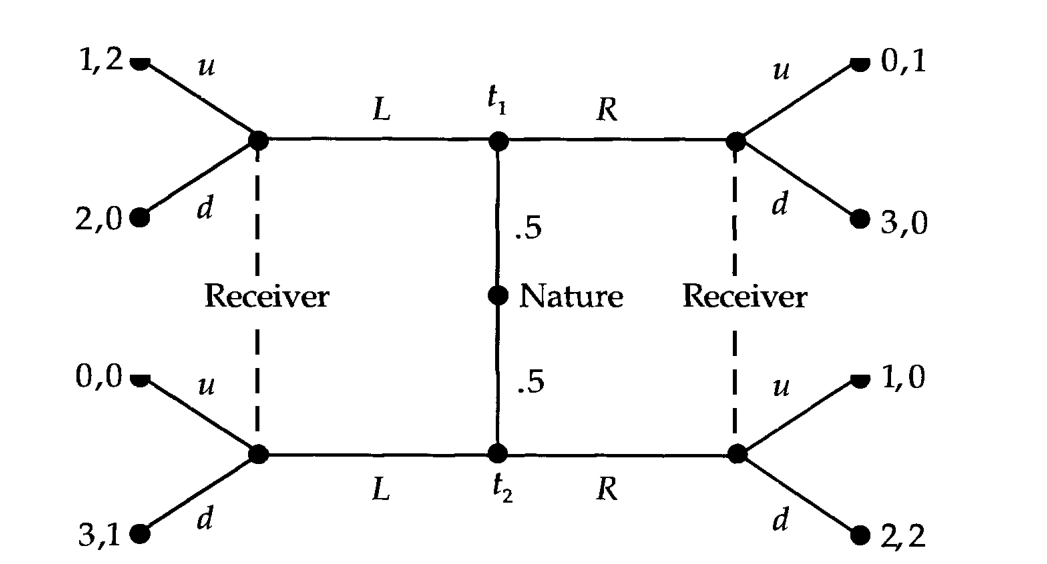
\includegraphics[keepaspectratio,alt={Problem 4.3(a) signaling game}]{../figures/gibbons-4-3a.png}}



\begin{enumerate}

\def\labelenumi{\alph{enumi}.}

\setcounter{enumi}{1}

\tightlist

\item

  The following three-type signaling game begins with a move by nature, not shown in the tree, that yields one of the three types with equal probability. Specify a pooling perfect Bayesian equilibrium in which all three Sender types play \(L\).

\end{enumerate}



\pandocbounded{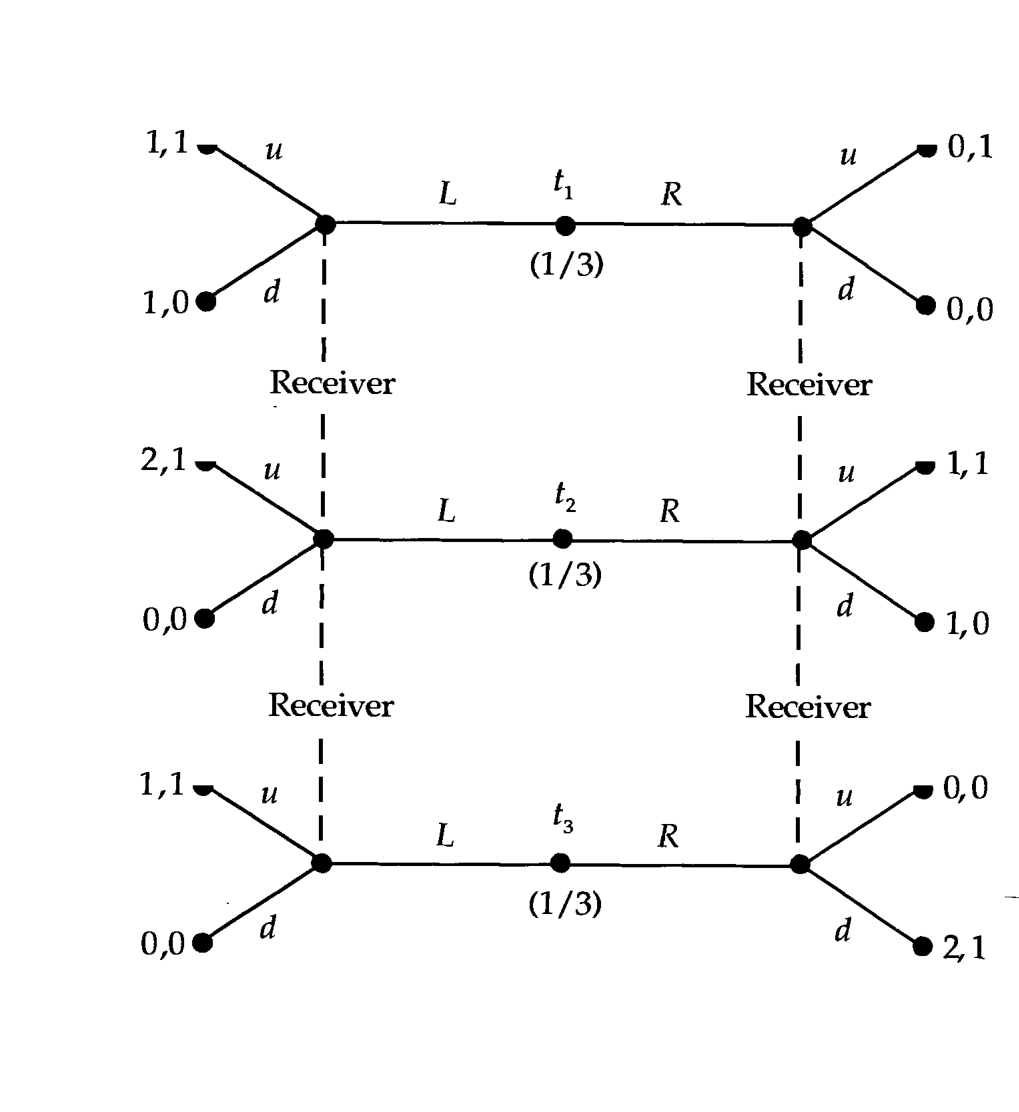
\includegraphics[keepaspectratio,alt={Problem 4.3(b) three-type signaling game}]{../figures/gibbons-4-3b.png}}

\end{quote}

